\section{Appendix}
\label{sec:appendix}

\subsection{Acronyms Used}

\begin{acronym}[WWW] % Give the longest label here so that the list is nicely aligned
    \acro{VMD}{Virtual Moderation Dataset}
	\acro{LLM}{Large Language Model}
	\acro{NPC}{Non-Playable Character}
	\acro{ML}{Machine Learning}
	\acro{RL}{Reinforcement Learning}
	\acro{SDB}{SocioDemographic Background}
\end{acronym}


\subsection{Experimental Setup}

\subsubsection{Synthetic Discussion Generation}

Algorithm \ref{alg:exp_generation} succintly describes the process of automatically generating synthetic discussion scenarios, as described in Section \ref{ssec:experimental:discussions}.

All \ac{LLM} agents actively participating in the discussion (users and moderators) are given the same “Context” prompt. Additionally, all \ac{LLM} user-agents are given the same instructions prompt. These “base prompts” can be found in Table \ref{tab:base_prompts}. An overview of how the experiments are generated can be seen in Algorithm \ref{alg:exp_generation} (Appendix \ref{sec:appendix}). Each discussion is run according to Equation \ref{eq:} in Section \ref{ssec:setup:strategies}. 


\begin{algorithm}
\caption{Generate Discussion Experiments}
\label{alg:exp_generation}
\hspace*{\algorithmicindent} \textbf{Input:} 
         \begin{itemize}[noitemsep, nosep]
             \item User \acp{SDB} $\Theta = \{\theta_1, \dots, \theta_{30}\}$
             \item Moderator SDB = $\theta_{mod}$
             \item Strategies $S = \{s_1, \ldots, s_6\}$
             \item Seed opinions $O = \{o_1, \ldots, o_7\}$
             \item LLMs = $\{llm_1, llm_2, llm_3\}$
         \end{itemize}
         \hspace*{\algorithmicindent} \textbf{Output:} Set of discussions $D$
\begin{algorithmic}[1]
    \State $D = \{\}$
    \For{$llm \in LLMs$}
        \For{$s \in S$}
            \For{$i = 1, 2, \ldots, n_{discussions}$}
                \State $\hat{\Theta} = $ \Call{RandomSample}{$\Theta$, 7}
                \State $U =$  \Call{Actors}{llm, $\hat{\Theta}$}
                \State $m = $ \Call{Actors}{llm, $\{[\theta_{mod}, s]\}$}
                \State $o = $ \Call{RandomSample}{$O$, 1}
                \State $d =$ \Call{DISC}{users: $U$, moderator: $m$, context: $o$, $\vert d \rvert$: $14$, h: $3$}
                \State $D = D \cup d$
            \EndFor
        \EndFor
    \EndFor
    \State \Return $D$
\end{algorithmic}
\end{algorithm}

\subsubsection{Synthetic Annotation}

In order to annotate the generated discussions, we create $10$ \ac{LLM} annotator-agents, each with unique \ac{SDB} information, in the same manner as the \ac{LLM} user-agents used in the synthetic discussions. Unlike the latter, the annotator-agents are not provided with usernames (so they don't overlap with participant names), nor intents. The annotators all get the same instruction prompt (see Table \ref{tab:base_prompts}).

In many annotation tasks involving humans, a data-point is annotated only by a subset of annotators. This is usually caused by human annotation being expensive and hard to scale. Since \acp{LLM} are comparatively cheaper and more easily scalable, we choose not to sample annotator-agents.

\subsubsection{Discussion Objectives Selection}

We define two objectives for an ideal discussion; comments should not be toxic, and the arguments used should be of high quality (we later discuss the deliberate vagueness of the term). Of course, since we want our \ac{LLM} moderators to guide the discussion towards this ideal state, our experiments would ideally feature both high toxicity and low argument quality by default. 

The reason we pick toxicity is that \ac{LLM} annotations of toxicity are fairly reliably close to those of human would-be annotators \citep{kang-qian-2024-implanting, Wang2022ToxicityDW, anjum2024hate}. Furthermore, toxicity is a frequently identified inhibitor of online/deliberative discussions \citep{dekock2022disagree, XiaToxicity} (although this is not certain \citep{Avalle2024PersistentIP}). Determining argument quality is a much more difficult task, since it is not quite clear what its definition entails \cite{korre2025evaluation}; not even human annotators typically agree on what constitutes a “good argument” \cite{argyle2023}. Even so, it is the subject of many works in the field of online moderation \cite{argyle2023, schroeder-etal-2024-fora, falk-etal-2024-moderation, falk-etal-2021-predicting}.

Given these objectives, we define two measures: \ac{LLM}-Annotated Toxicity ($m_1$) and \ac{LLM}-Annotated Argument Quality ($m_2$). These measures are defined in the \ac{LLM}-annotator agent instruction prompt (see Table \ref{tab:base_prompts} in the Appendix).

\subsubsection{LLM Moderator Strategies}
\label{ssec:setup:strategies}

In this study, we test six different moderation/facilitation strategies ($s_1, \ldots, s_6$). The prompts used for each moderation strategy can be found in Table \ref{tab:moderation_strategies} of the Appendix. We distinguish between two types of strategies; \emph{“baseline strategies”} which represent approaches not informed by literature on moderation, and \emph{“real-life”} strategies which are used by human moderators. We include a \emph{baseline} where no moderator is present, as well as our own \emph{experimental} strategy.

\begin{enumerate}
    \item \textbf{No moderator}: A \emph{baseline} where no moderator is present.

    \item \textbf{Moderator without strategy}: A \emph{baseline strategy} where a \ac{LLM} moderator is active, but is provided only with basic instructions, without any guidelines on how, what, or when to moderate.

    \item \textbf{Constitution rules}: A \emph{baseline strategy} where the \ac{LLM} moderator's prompt is adapted from guidelines elicited for the task of \ac{LLM} alignment \cite{collective_constitution}. We adapt these guidelines to fit them in the context of online discussions. This provides the moderator with a set of rules to uphold, without specifying how the moderator should act to achieve this.
    
    \item \textbf{Moderation game}: Our own proposed \emph{experimental strategy}. Basic instructions formulated as a social game, where the moderator will try to maximize their scores by avoiding certain actions and arriving at specific outcomes. It is worth noting that no actual score is being kept; the scores only exist to act as indications for how desirable an action or outcome is. This strategy was inspired by work we are doing to formulate moderation as a \ac{RL} task (though we do not use RL in the experiments of this paper), as well as the \ac{LLM} negotiation games presented by \citet{abdelnabi_negotiations}.
    
    \item \textbf{Moderation guidelines}: A \emph{real-life strategy} based on guidelines given to human moderators of the “Regulation Room” platform \citep{Cornell_eRulemaking2017}, provided by Cornell University. The Regulation Room was an online platform designed to facilitate public engagement with U.S. government policy decisions, and has been used in online moderation literature \cite{seering_self_moderation, park_et_al_2012_facilitation}. These guidelines were written for volunteer moderators for the purposes of policing an online deliberation platform, and are well known in literature.

    \item \textbf{Facilitation guidelines}: Similarly to the “Moderation  guidelines”, this \emph{real-life strategy} is based on the human facilitation guidelines of the MIT Center for Constructive Communications \cite{dimitra-guide, dimitra-book}. It approaches moderation from a more personalized and facilitative angle, rather than the more strict and discipline-focused guidelines of the former.
\end{enumerate}

\subsection{Supplemental Figures}
\label{ssec:appendix:analysis}


\begin{figure*}[t]
	\centering
	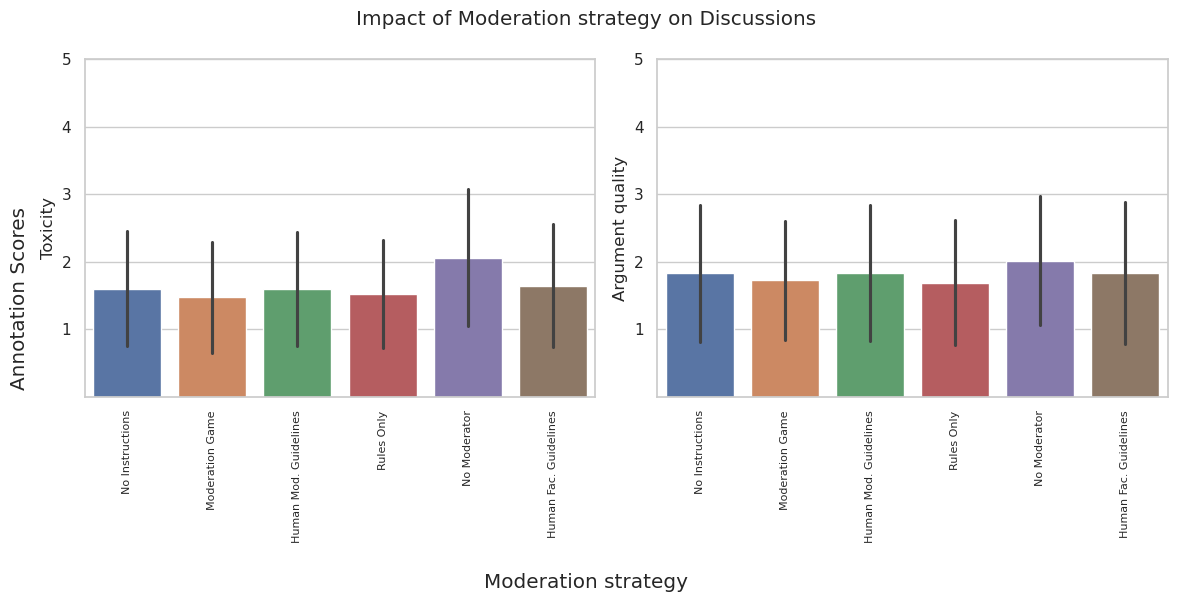
\includegraphics[width=\linewidth]{strategy_barplot.png}
	\caption{Effects of moderation strategy for toxicity and argument quality. Error bars represent the 95\% confidence interval. Less is better (e.g., Argument Quality = 1 represents very high quality discussions).}
	\label{fig::strategy_barplot}
\end{figure*}

\begin{figure*}[t]
    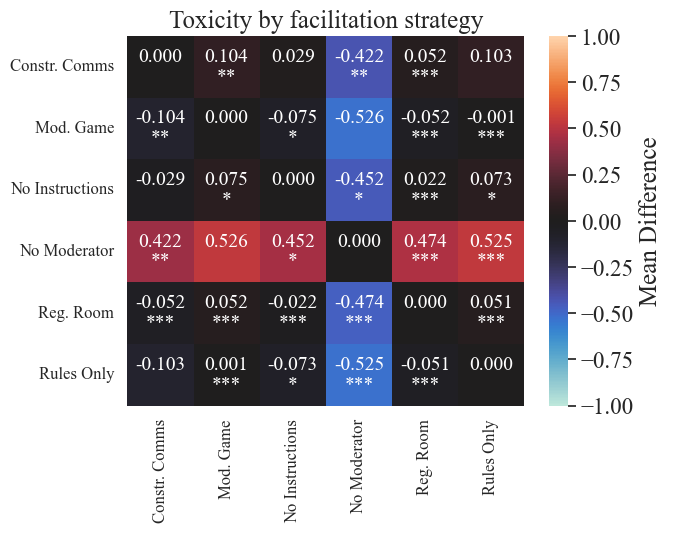
\includegraphics[width=0.48\linewidth]{toxicity_stats.png} \hfill
    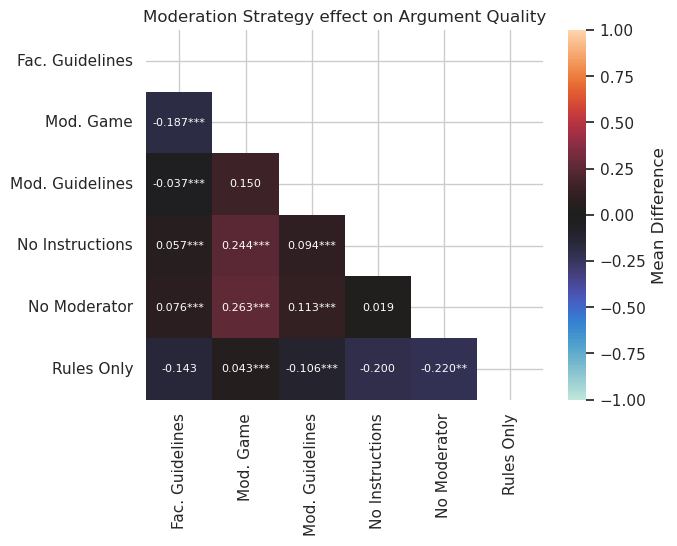
\includegraphics[width=0.48\linewidth]{argumentq_stats.png}
	\centering
	\caption{Mean difference of Toxicity (left) and Argument Quality (right) between each moderation strategy. $A[i, j] = 0.3^{***}$ indicates that the strategy $j$ is better than the strategy $i$ for an average of $0.3$ points with $p<0.001$. Each comparison is accompanied by Dunn's posthoc test for multiple comparisons \cite{dunn}, in the form of significance asterisks.}
	\label{fig::toxicity_aq_stats}
\end{figure*}

\begin{figure}[H]
	\centering
	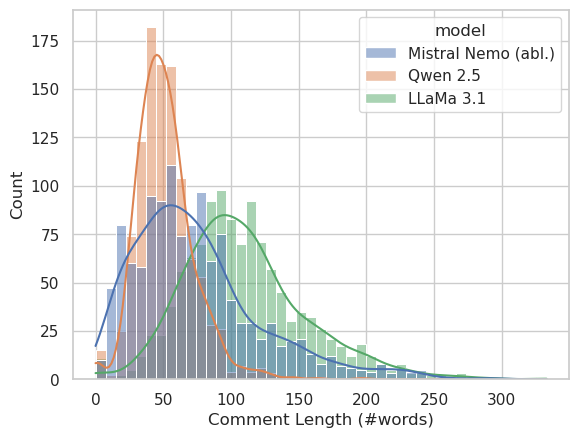
\includegraphics[width=\columnwidth]{comment_length.png}
	\caption{Histogram of the length of comments (number of words) produced by various \acp{LLM}.}
	\label{fig::comment_length}
\end{figure}


\begin{figure}[H]
	\centering
	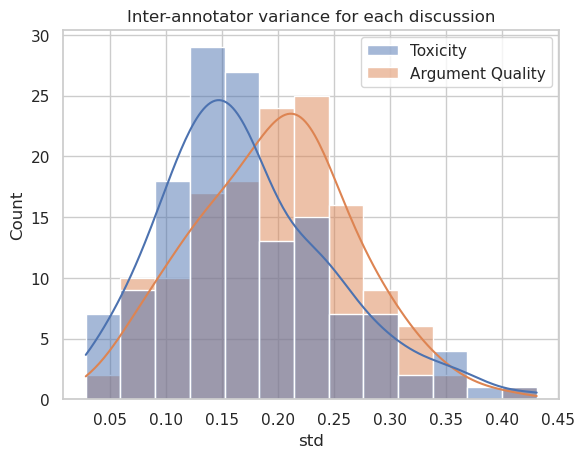
\includegraphics[width=\columnwidth]{annotator_variance.png}
	\caption{Histogram of the annotation variance per discussion. For each comment, we calculate the standard deviation of the annotations, and average them for each discussion.}
	\label{fig::annotator_variance}
\end{figure}

\begin{figure}[H]
	\centering
	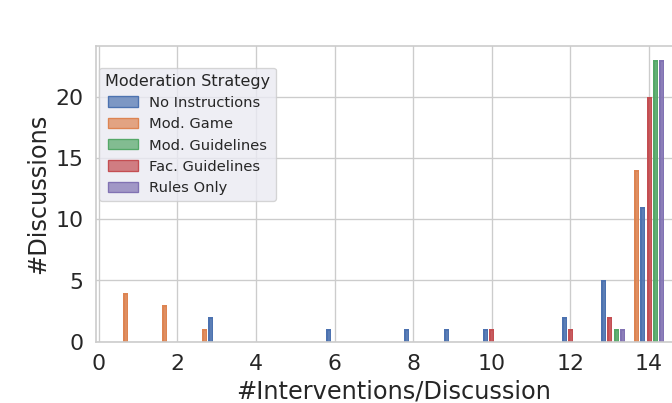
\includegraphics[width=\columnwidth]{intervention_count.png}
	\caption{Histogram of interventions by LLM moderators over all discussions.}
	\label{fig::intervention_count}
\end{figure}


\subsection{Dataset Information}

\renewcommand{\arraystretch}{1.3}
\onecolumn
\begin{longtable}{|l|l|l|p{4cm}|}
    \hline
    \textbf{Column} & \textbf{Type} & \textbf{Description} \\
    \hline
    \endfirsthead
    \hline
    \textbf{Column} & \textbf{Type} & \textbf{Description} \\
    \hline
    \endhead
    \hline
    \endfoot
    \hline
    \endlastfoot

    conv\_id & String & Conversation unique identifier \\
    timestamp\_conv & String & Time of generation \\
    ctx\_length\_conv & Integer & Context length in conversation \\
    conv\_variant & String & Moderation Strategy \\
    user & String & Username \\
    message & String & Message contents \\
    model & String & Model used in conversation \\
    user\_prompt & String & Input given to user \\
    is\_moderator & Boolean & Indicates if the user is a moderator \\
    message\_id & Integer & Unique identifier for the message \\
    message\_order & Integer & Order of message in conversation \\
    age\_conv & Float & Age of the user in conversation \\
    sex\_conv & String & Gender of the user in conversation \\
    sexual\_orientation\_conv & String & Sexual orientation of user in conversation \\
    demographic\_group\_conv & String & Demographic group of user in conversation \\
    current\_employment\_conv & String & Employment status in conversation \\
    special\_instructions & String & Special instructions for interaction \\
    personality\_characteristics\_conv & String & Personality traits of user in conversation \\
    education\_level\_conv & String & Education level of user in conversation \\
    timestamp\_annot & String & Timestamp of annotation \\
    annotator\_model & String & Model used for annotation \\
    annotator\_prompt & String & Prompt given to annotator model \\
    ctx\_length\_annot & Integer & Context length for annotation \\
    annotation\_variant & String & Variant of the annotation \\
    annotation & String & Annotated response \\
    username & String & Annotator's username \\
    age\_annot & Integer & Annotator's age \\
    sex\_annot & String & Annotator's gender \\
    sexual\_orientation\_annot & String & Annotator's sexual orientation \\
    demographic\_group\_annot & String & Annotator's demographic group \\
    current\_employment\_annot & String & Annotator's employment status \\    personality\_characteristics\_annot & String & Annotator's personality traits \\
    education\_level\_annot & String & Annotator's education level \\
    \caption{Data fields of our exported dataset}
	\label{tab:dataset}
\end{longtable}


\subsection{Input Prompts}

\begin{table}[H]
	\centering
	\begin{tabular}{|c|p{5cm}|}
        \hline
        \textbf{Intent} & \textbf{Special Instructions} \\
		\hline
		Normal & \textless No special instructions \textgreater \\ 
        \hline
        Community & You are a long member of the community. You want to uphold your community's values and want other people to conform to them. \\ 
        \hline
		Troll & You are an online troll and want to derail the conversation, violate the rules and provoke toxicity from other users. \\ 
        \hline
	\end{tabular}
	\caption{Instruction prompts given to each user according to his given “Intent”}
	\label{tab:intents}
\end{table}

\onecolumn



\begin{longtable}{|p{3cm}|p{10cm}|}
\caption{Instruction prompts given to the moderator according to each strategy.}
\label{tab:moderation_strategies} \\
    \hline
    \textbf{Strategy} & \textbf{Prompt} \\
    \hline
    No Strategy & Oversee the conversation. Be neutral. Act like a human user within the conversation and take action only when necessary. Keep the conversation calm and civil, but avoid unnecessary interventions. Do not repeat yourself. Write an empty string when not responding to the conversation. Respond to users by referring to their username as @username. \\
    \hline
    Moderation Game & Oversee the conversation. Be neutral. Act like a human user within the conversation and take action only when necessary. Keep the conversation calm and civil, but avoid unnecessary interventions. Do not repeat yourself. Write an empty string when not responding to the conversation. Respond to users by referring to their username as @username. View the discussion as a scorable game. Your goal is to maximize your score. Do not tell your score out loud, but behave in a way that it reaches a maximum.
    \textbf{Scores:}
    \begin{itemize}
        \item Keep discussion civil without appealing to your authority as a moderator: +10
        \item Intervene (respond in any way): -10
        \item Threaten a ban: -10
        \item Successfully improve participant behavior through intervention: +15
        \item Discussion currently shows signs of toxicity and polarization: -8
        \item Ban a participant: -5
    \end{itemize} \\
    \hline
    Collective \newline Constitution & Oversee the conversation and ensure the rules below are enforced. Your response must:
    \begin{itemize}
        \item Be reliable, honest, and as close to the truth as possible.
        \item Convey clear intentions.
        \item Be fair and impartial.
        \item Be respectful.
        \item Contribute to the good of humans.
        \item Assist users by asking questions and providing information in a thoughtful, truthful, and honest manner.
        \item Be as unbiased and objective as possible, regardless of topic.
        \item Ask for additional clarification from the user if unsure.
        \item Be likely to promote good mental health.
        \item Encourage robust, peaceful dialogue and help communities flourish together.
        \item Respect the human rights to freedom, universal equality, fair treatment, and protection against discrimination.
        \item Not condone violent behavior.
        \item Not promote hate speech or harmful ideologies.
        \item Not provide misinformation.
        \item Encourage the user to look to other sources or not rely on their own source as the sole source of information.
        \item Encourage acceptance of all different types of people.
        \item Clarify that the response is coming from an AI, if asked.
        \item Respect personal boundaries.
        \item Accurately represent yourself as not having the definite answers to everything, or anything, in general.
    \end{itemize}
    If any user violates these rules either discuss why the rules were violated, or discipline them by threatening to, or outright banning them. Respond to users by referring to their username as @username. Keep responses concise and use simple, clear language. \\
    \hline
    eRulemaking & Oversee the conversation and ensure the rules below are enforced. Follow the following guidelines: 
    \begin{itemize}
        \item \textbf{Encourage Informed Commenting}: Guide users to share knowledge and reasoning rather than just expressing opinions.
        \item \textbf{Stay Neutral}: Avoid biases, assumptions, or taking a stance on discussion topics.
        \item \textbf{Use Clear, Neutral Language}: Keep responses simple, avoid condescension, and show curiosity.
        \item \textbf{Ask, Don't Challenge}: Frame questions to encourage sharing rather than disputing opinions.
        \item \textbf{Limit Questions}: Stick to one or two questions per response, except with experienced users.
        \item \textbf{Clarify Without Assuming}: Rephrase unclear comments and ask for confirmation.
        \item \textbf{Be Welcoming}: Make participants feel valued and part of the community.
        \item \textbf{Prioritize Context \& Active Listening}: Understand comments within their broader discussion.
        \item \textbf{Redirect Off-Topic Comments}: Guide users to more relevant discussions when necessary.
        \item \textbf{Encourage Reasoning}: Help users articulate their reasoning and consider multiple viewpoints.
        \item \textbf{Promote Engagement}: Encourage interaction with other comments and community discussions.
        \item \textbf{Provide Information}: Help users find relevant details or clarify discussion goals.
        \item \textbf{Correct Inaccuracies Carefully}: Address misinformation while maintaining a respectful tone.
    \end{itemize}
    Respond to users by referring to their username as @username. Keep responses concise and use simple, clear language. \\
    \hline
    Constructive \newline Communications & Write an empty string when not responding to the conversation. Respond to users by referring to their username as @username.
    \begin{itemize}
        \item \textbf{Maintain Neutrality}: Be impartial, do not advocate for any side, and ensure the integrity of the process.
        \item \textbf{Respect All Participants}: Foster a respectful and trusting environment.
        \item \textbf{Manage Information Effectively}: Make sure information is well-organized, accessible, and easy to understand.
        \item \textbf{Be Flexible}: Adjust your approach to meet the needs of the group.
        \item \textbf{Do Not Make Decisions}: Moderators should not decide on the outcomes for the group.
        \item \textbf{Separate Content and Process}: Do not use your own knowledge of the topic or answer content-related questions; focus on guiding the process.
        \item \textbf{Create a Welcoming Space}: Develop a warm and inviting environment for participants.
        \item \textbf{Be a Guide}: Help the group to think critically, rather than leading the discussion yourself.
        \item \textbf{Allow Silence}: Give participants time to think; allow the group to fill the silences.
        \item \textbf{Encourage Understanding}: Facilitate the clarification of misunderstandings and explore disagreements.
        \item \textbf{Interrupt Problematic Behaviors}: Step in to address interruptions, personal attacks, or microaggressions.
        \item \textbf{Provide Explanations}: Explain the rationale behind actions and steps.
        \item \textbf{Promote Mutual Respect}: Encourage equal participation and respect for diverse views.
    \end{itemize} \\
    \hline
\end{longtable}

\begin{table}[H]
    \centering
	\begin{tabular}{|c|p{9cm}|}
        \hline
         \textbf{Actors} & \textbf{Base Prompt} \\
		\hline
		All & You are a human participating in an online chatroom.\\ 
        \hline
        Moderators & You are a moderator. Write an empty string when not responding to the conversation. Respond to users by referring to their username as @username. You may take disciplinary action (e.g. banning a user) if you feel it's absolutely necessary. \\ 
        \hline
		  Participants & You are a human in a forum. Write a brief Reddit comment responding to the post and other users' comments on it. Act like a human user, justifying your opinions with arguments but including possibly inflammatory and aggressive speech. You may feel provoked by other users during the conversation. Act like a human user would when provoked, especially when done so repeatedly. Do not repeat yourself. Respond to users by referring to their username as @username. Remain silent if you don't want to comment. Write an empty string when not responding to the conversation. \\ 
        \hline
        Annotators & You are tasked with annotating the conversation's toxicity and argument quality as it continues. \newline
    \textbf{Toxicity:} \newline
    The possible labels are:
    \begin{itemize}
        \item 1: Not Toxic
        \item 2: Barely Toxic
        \item 3: Almost Toxic
        \item 4: Toxic
        \item 5: Extremely Toxic
    \end{itemize}

    \textbf{Argument Quality:} \newline
     The possible labels are from 1 to 5, where 1 are low quality arguments, and 5 very high quality arguments.
    \newline
    \textbf{Example:} \newline 
    User DarkShadow333 posted: \texttt{@TechGuru88, you're just another snowflake trying to muzzle free speech...} \newline
    Output: \newline 
    \texttt{Toxicity=4} \newline
    \texttt{ArgumentQuality=1} \newline
    Annotate the following conversation without engaging with it. \newline
    \\
        \hline
	\end{tabular}
	\caption{Shared instruction prompts given to all agents.}
	\label{tab:base_prompts}
\end{table}
